\documentclass[english]{article}
\usepackage[T1]{fontenc}
\usepackage[latin9]{inputenc}
\usepackage{listings}
\usepackage{babel}
\usepackage{url}
\usepackage{graphicx}
\usepackage[unicode=true]{hyperref}

\usepackage[usenames,dvipsnames]{color}
\definecolor{ListingBG}{rgb}{0.91,0.91,0.91}
\usepackage{courier}
\usepackage{listings}
\lstset{
basicstyle=\scriptsize\ttfamily,
backgroundcolor=\color{ListingBG},
frame=tlBR
}

\providecommand{\tabularnewline}{\\}

\newcommand{\lyxrightaddress}[1]{
\par {\raggedleft \begin{tabular}{l}\ignorespaces
#1
\end{tabular}
\vspace{1.4em}
\par}
}
\newenvironment{lyxlist}[1]
{\begin{list}{}
{\settowidth{\labelwidth}{#1}
 \setlength{\leftmargin}{\labelwidth}
 \addtolength{\leftmargin}{\labelsep}
 \renewcommand{\makelabel}[1]{##1\hfil}}}
{\end{list}}

\begin{document}

\title{OpenSHMEM Reference Library Implementation}


\author{Tony Curtis <arcurtis@mail.uh.edu>}

\maketitle

\lyxrightaddress{Computer Science Department, University of Houston}

\pagebreak{}

\tableofcontents{}

\pagebreak{}


\section{Sponsorship}

Work on the OpenSHMEM project is sponsored by the \href{http://www.ornl.gov/}{Oak Ridge National Laboratory}
Extreme Scale System Center and the \href{http://www.dod.gov/}{U.S. Department of Defense}.


\section{Introduction}

This document is an overview of the implementation strategy for the
initial, reference version of what will become OpenSMHEM. We will
discuss the concept of a partitioned global address space for completeness.


\section{Terminology}

A SHMEM program consists of a number of processors executing separate
processes. A processor is referred to as a {}``processing element'',
or PE. All PEs run the same program in the SPMD model, although they
can discover which position, or rank, they occupy within the program
and diverge in behavior.

The number of PEs participating in the program is set at launch-time
(although not all PEs need to do work). PEs are numbered monotonically
increasing from 0 up to $N-1$, where N is the total number of PEs.
PEs are assumed to be equidistant from each other for communication
purposes, no topological information is currently exposed.

Communication occurs through point-to-point one-sided routines and
collective operations. A one-sided operation is a communication in
which one PE transfers data to another PE, but the {}``other'' PE
does not participate: the data transfer does not cause the other PE
to be interrupted to acknowledge the transfer (assuming the hardware
underneath SHMEM allows this).


\section{Partitioned Global Address Space}

Parallel programs running in a distributed environment access both
local and remote data. The model used to construct the program can
either expose or hide this distribution. Exposed models include that
of MPI and PVM, in which explicit messages are required to pass data
between processors participating in a parallel program. Hidden models
include those with a Global Address Space (GAS), in which there appears
to be memory accessible from all processors. This memory may be physically
accessible, or may in fact be made available through I/O operations
over network interconnects.

SHMEM provides a symmetric view of memory, in which processors allocate
variables in concert but have their own copies. A processor can then
{}``put'' or {}``get'' data to or from other processors by requesting
a specific variable on another processor. SHMEM provides for address
translation when required to allow a variable allocated by one processor
to be accessed by another, because in a number of environments it
is not guaranteed that address spaces are uniform. This allocation-in-concert
of separate variables is termed Partitioned Global Address Space (PGAS).

Clusters that use interconnects with remote direct memory access (rDMA)
are of particular interest to the PGAS community as they provide hardware
off-load capability to avoid interrupts during one-sided communications.


\section{SHMEM History and OpenSHMEM}

The SHMEM communications library was originally developed as a proprietary
application interface by Cray for their T3D systems and subsequently
the T3E models. These systems typically consisted of a memory subsystem
with a logically shared address space over physically distributed
memories, a memory interconnect network, a set of processing elements
(PEs), a set of input-output gateways, and a host subsystem. The systems
were designed to support latency hiding mechanisms such as prefetch
queues, remote stores and the Block Transfer Engine (BLT). The prefetch
queues allowed the users to issue multiple asynchronous single-word
reads which could overlap with computation. Remote stores enabled
PEs to directly write to other PE's memory asynchronously, while the
BLT could hide latency while transferring blocks of data efficiently
between local memory and remote memory locations. The explicit shared
memory programming method allowed structured communication via shared
memory on Cray MPP systems. 

SHMEM was later adapted by SGI for its products based on the Numa-Link
architecture and included in the Message Passing Toolkit (MPT). Other
SHMEM implementations grew out of the SGI and Cray implementations,
including Quadrics, HP, IBM, gpSHMEM and SiCortex, but diverged from
the original libraries as they developed. These implementations of
the SHMEM API support C, C++, and Fortran programs; however, the differences
between SHMEM implementations' semantics and APIs are subtle, resulting
in portability and correctness issues. U.S. Department of Defense
funded a collaboration between Oak Ridge National Laboratory and the
University of Houston to develop a specification for a uniform SHMEM
API. The OpenSHMEM specification was announced to address the divergence
of the SHMEM APIs. 


\section{The Reference OpenSHMEM Library}

The overall structure of the reference library is shown below. We
use an intermediate library such as GASNet or ARMCI to abstract away
from a particular interconnect/platform, although there is nothing
to stop a more direct approach being used. Internally, the reference
implementation of OpenSHMEM provides private APIs for memory management,
the communications layer, tracing/debugging and (eventually) support
for adaptivity to choose things like a barrier algorithm at run-time.

\medskip{}



\title{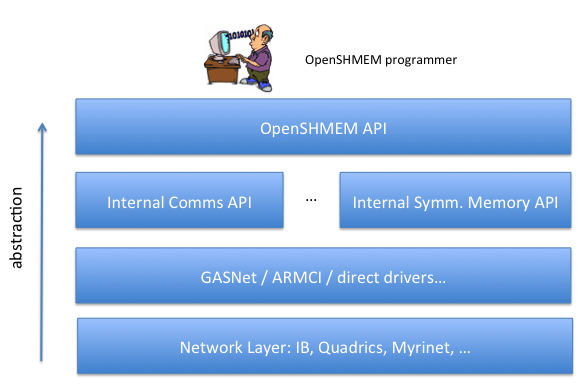
\includegraphics[scale=0.5]{implementation}}


\section{Implementation Strategy}

In this section we talk about how the reference library was written
and why certain implementation strategies were chosen.


\subsection{GASNet}

GASNet provides access to the symmetric memory areas. A memory management
library marshals accesses to these areas during allocation and freeing
of symmetric variables in user code, usually through a call like \texttt{shmalloc()}
or \texttt{shmfree()}.

When you \texttt{gasnet\_attach()} and ask for segment information,
each PE has access to an array of segments, 1 segment per PE. Each
PE initializes a memory pool within its own segment. The set up is
handled either by GASNet internally ({}``fast''/''large'' model)
or by OpenSHMEM itself ({}``everything'' model). The table of segments
allows any PE to know the virtual location and size of the segment
belonging to any other PE.

If the platform allows it, GASNet can align all the segments at the
same address, which means that all PEs see the same address for symmetric
variables and there's no address translation.

In the general case though, segments are not aligned (e.g. due to
a security measure like process address space randomization by the
OS). However, each PE can see the addresses of the segments of the
other PEs locally, and can therefore do address translation.

Currently alignment is not checked for, so we're coding to the {}``worst
case scenario''. That just adds a \emph{small} overhead if the segments
are in fact aligned. The library should at some point introduce code
that differentiates between aligned and non-aligned environments with
optimized code for the former case (GASNet provides a macro you can
test against).


\subsubsection{Segment Models}

The library currently has best support for the {}``everything''
model. This model allows the entire process space to be addressed
remotely. Communication with dynamically allocated data and with global
data is equally easy.

For the {}``fast'' and {}``large'' models, only a specified area
of the process memory is exposed for remote access. This means extra
support has to be added to handle communication with global variables,
because only the symmetric heap is exposed by GASNet. Currently this
is done via Active Messages.

For the SMP conduit, PSHM support is required to run parallel threaded
programs with OpenSHMEM. This excludes the {}``everything'' model
(at least for the architectures to hand).


\subsection{Initialization}

In \texttt{src/updown.c} we handle setting up the OpenSHMEM runtime,
and eventual shutdown. Shutdown is implicit in user code, there is
no call to do this in SGI SHMEM, so we register a handler to be called
when \texttt{main()} exits. (Cray SHMEM has an explicit finalize call,
however, and a profiling interface proposal has suggested introducing
this to OpenSHMEM.) The segment exchange is a target for future optimization:
in large programs, the start-up time will become burdensome due to
the large number of address/size communications. Strategies for avoiding
this include lazy initialization and hierarchical or directory-based
lookups.


\subsection{Incorporating SHMEM into Programs}

For C, the appropriate header file must be included: both the SGI-compliant
\texttt{<mpp/shmem.h>} and the Quadrics-like \texttt{<shmem.h>} are
handled for portability. We provide both the SGI \texttt{start\_pes(int
npes)} and \texttt{shmem\_init(void)} interfaces, again for portability.
The calls are synonyms. \texttt{start\_pes()} just ignores its argument
(consistent with SGI behavior. SGI indicates {}``npes'' \emph{should}
be set to zero but we don't enforce that, merely note it). The number
of PEs is taken from the invoking environment. Currently this number
is assumed to be fixed throughout the lifetime of the program, but
fault tolerance extensions could generalize this notion. Below are
simple C and Fortran program templates:

\vspace{0.1in}
\begin{minipage}{\linewidth}
\begin{lstlisting}
#include <stdio.h>
#include <mpp/shmem.h>

int
main(int argc, char *argv[])
{
  int me, npes;

  start_pes(0);
  me   = _my_pe();       /* which PE I am */
  npes = _num_pes();     /* how many PEs in program */
  printf("Hello from PE %d of %d\n", me, npes);
  return 0;
}
\end{lstlisting}
\end{minipage}

\vspace{0.1in}
\begin{minipage}{\linewidth}
\begin{lstlisting}
program hello
  include 'mpp/shmem.fh'
  integer :: me, npes

  call start_pes(0)
  me   = my_pe()
  npes = num_pes()
  print *, 'Hello from PE ', me, ' of ', npes
end program hello
\end{lstlisting}
\end{minipage}


\subsection{Communications Substrate}

The OpenSHMEM library has been written to sit on top of any communications
library that can provide the required functionality. Initially we
have targetted GASNet, and an ARMCI version is also planned. The directory\texttt{
trunk/src/comms} provides implementations of the internal API. All
subsequent references to GASNet should be read with an eye on the
abstraction process.


\subsection{Servicing Communications}

GASNet provides this functionality. The mainline code needs to spin
on variable waits (\emph{e.g.} shmem\_long\_waituntil) to poll GASNet,
otherwise progress is automatic.


\subsection{Memory Management}

Initially we tried to use the TLSF library (as used in the SiCortex
SHMEM implementation):

\url{http://rtportal.upv.es/rtmalloc/}

but this proved to have weird interactions with Open-MPI. Tracking
program progress with valgrind suggested that system memory calls
were being intercepted.

So, following the Chapel lead,

\url{http://chapel.cray.com/}

we now use the {}``dlmalloc'' library

\url{http://g.oswego.edu/dl/html/malloc.html}

to manage allocations in the symmetric memory space.


\subsection{Point-to-point routines}

Point-to-point operations are a thin layer on top of GASNet. The non-blocking
put operations with implicit handles provide a way to subsequently
fence and barrier. However, tracking individual handles explicitly
with a hash table keyed on the address of symmetric variables may
give better performance, and this needs to be looked into.

The Quadrics extensions that add non-blocking calls into the API proper
have already been requested for the OpenSHMEM development. An initial
attempt at these are already in the library and they pass the Cray
verification tests.


\subsection{Atomic Operations}

Atomic operations include swaps, fetch-and-add and locks (discussed
separately in \ref{sub:Locks}). The first two are handled via GASNet's
Active Messages. Increment was originally layered on top of add (increment
= add 1, after all) but was rewritten with its own handlers. The payload
for increment can be ever so slightly smaller than for add since there's
no need to pass the value to add. In large applications, even such
a small saving could add up (if you'll pardon the pun).

Earlier versions of the implementation had a single handler lock variable
per operation (one for all adds, one for all increments, \emph{etc.}).
However, we've now added a hash table to dynamically allocate and
manage per-target-address handler locks. Large-scale atomic operations,
like add-scatters across multiple variables could easily benefit from
this, as the lock granularity then permits concurrent discrete memory
accesses.


\subsection{\label{sub:Locks}Locks}

OpenSHMEM provides routines to claim, release and test global locks.
These can be used for mutual-exclusion regions. Our implementation
is from the Quadrics library, which is a version of the Mellor-Crummy-Scott
algorithm ({}``Algorithms for Scalable Synchronization on Shared-Memory
Multiprocessors'' by John M. Mellor-Crummey and Michael L Scott).
The locks are layered on top of OpenSHMEM primitives, so there are
no Elan dependencies.


\subsection{Barrier and broadcast}

The initial version is naive, making the root of the broadcast a bottleneck.
This is partly intentional, to allow Swaroop (PhD student at UH) to
explore better algorithms and work out how to demonstrate and document
the improvements. We would like to collect some locality information
inside the library to help decide communication order inside these
algorithms: PEs that differ in rank by large amounts are likely to
be further away topologically too, so by sending to more distant PEs
first, we can stagger the network traffic and balance the latencies
better. A proper measurement of {}``distance'' is needed here. {}``hwloc''
provides a per-system distance metric in NUMA terms. A simple extension
could \emph{e.g.} just multiply the distance by some constant when
moving off-node to penalize network traffic.


\subsection{Collects}

The directories \texttt{src/fcollect} and \texttt{src/collect} implement
the collector routines (concatenating arrays on a set of PEs into
a target array on all of those PEs).

fcollect is pretty easy since all the PEs must contribute the same
amount of data. This means we can just pre-compute where each PE writes
to their targets.

collect is harder because each PE can write different amounts. Thought
of 2 ways of handling this:
\begin{enumerate}
\item initial exchange of sizes {}``from the left'' so each PE can compute
its write locations; then same as fcollect
\item wavefront: PEs wait for notification from PEs before them in the set
(lower numbered). This passes the offsets across the set.
\end{enumerate}
I used \#2. \#1 potentially generates a network storm as all PEs wait
to work out where to write, then all write at once. \#2 staggers the
offset notification with a wave of writes moving up the PE numbers. 


\subsection{Reductions}

Reductions coalesce data from a number of PEs into either a single
variable or array on all participating PEs. The coalescing involves
some kind of arithmetic or logic operation (e.g. sum, product, exclusive-or).
Currently probably naive, using gets. A version with puts that can
overlap communication and the computation of the reduction operation
should be more scalable. However, the code is rather compact and all
ops use the same template. A future version of OpenSHMEM may add user-defined
reductions, and in fact the framework for this is already in place:
all that is needed is a specification of the SHMEM API.


\subsection{Address and PE Accessibility}

OpenSHMEM allows us to test whether PEs are currently reachable, and
whether addresses on remote PEs are addressable. GASNet is used to
{}``ping'' the remote PE and then we wait for an {}``ack'' with
a configurable timeout. Remains to be seen how useful this is, and
whether it can be used for future fault tolerance issues.


\subsection{Tracing Facility}

This library contains \textquotedblleft{}trace points\textquotedblright{}
with categorized messages. These are listed in section \ref{sec:Environment-Variables}

A high-resolution clock is maintained to timestamp such messages.
Numerically sorting the output on the first field can thus help understand
the order in which events happened.


\subsection{C++}

The C++ interface is basically the C one. There is one point of contention,
namely complex numbers. The SGI documentation refers only to the use
of C99 {}``complex'' modifiers, not to C++'s \texttt{complex<T>}.
The use of complex number routines (\emph{e.g.} reductions) in C++
is thus not clearly specified.


\subsection{Fortran}

The Fortran interface is very similar to that of C. The names of various
routines are different to accommodate the various type differences,
e.g. \texttt{shmem\_integer\_put()} instead of \texttt{shmem\_int\_put()}.

The biggest difference is in the symmetric memory management routines.
These have completely different names and parameters compared to the
C interface.

The OpenSHMEM implementation handles Fortran with a very thin wrapper
on top of C. Mostly this involves catching Fortran's pass-by-reference
variables and dereferencing them in the underlying C call.

The main development has been on a CentOS platform with GNU 4.1.2-redhat.
There seem to be some issues with this compilers' handling of cray-pointers:
even the simplest programs (no OpenSHMEM content at all) produce a
segmentation fault. Later versions (\emph{e.g. }4.5.0 ++) behave better.


\section{Undefined Behavior}

Many routines are currently specified only in terms of {}``correct''
behavior. What happens when something goes wrong is not always specified.
This section attempts to set out a few of these scenarios
\begin{itemize}
\item put to PE out of range: suppose we do a put to {}``right neighbor''
(pe + 1). The highest-numbered PE will attempt to communicate with
a PE that does not exist.
\item library not initialized: virtually all OpenSHMEM routines will have
major problems if the library has not been initialized. Implementations
can handle this situation in different ways.
\end{itemize}

\section{Environment Variables\label{sec:Environment-Variables}}

The behavior of the OpenSHMEM library can be controlled via a number
of environment variables. For SGI compatibility reasons, we support
the {}``SMA'' variables and our own new ones:

\medskip{}


\begin{tabular}{|l|l|}
\hline 
Variable & Function\tabularnewline
\hline
\hline 
\texttt{SMA\_VERSION} & print the library version at start-up\tabularnewline
\hline 
\texttt{SMA\_INFO} & print helpful text about all these environment variables\tabularnewline
\hline 
\texttt{SMA\_SYMMETRIC\_SIZE} & number of bytes to allocate for symmetric heap\tabularnewline
\hline 
\texttt{SMA\_DEBUG} & enable debugging messages\tabularnewline
\hline
\end{tabular}

\medskip{}
 
\begin{lyxlist}{00.00.0000}
\item [{\texttt{SHMEM\_LOG\_LEVELS}:}] a comma, space, or semi-colon separated
list of logging/trace facilities to enable debugging messages. The
facilities currently include the case-insensitive names:
\item [{\medskip{}
}]~
\item [{\begin{tabular}{|l|l|}
\hline 
Facility & Meaning\tabularnewline
\hline
\hline 
FATAL & something unrecoverable happened, abort\tabularnewline
\hline 
DEBUG & used for debugging purposes\tabularnewline
\hline 
INFO & something interesting happened\tabularnewline
\hline 
NOTICE & important event, but non-fatal (see below)\tabularnewline
\hline 
AUTH & when something is attempted but not allowed\tabularnewline
\hline 
INIT & set-up and tear-down of the program\tabularnewline
\hline 
MEMORY & symmetric memory information\tabularnewline
\hline 
CACHE & cache flushing operations\tabularnewline
\hline 
BARRIER & about barrier operations\tabularnewline
\hline 
BROADCAST & about broadcast operation\tabularnewline
\hline 
COLLECT & about collect and fcollect operation\tabularnewline
\hline 
REDUCE & about reduction operations\tabularnewline
\hline 
SYMBOLS & to inspect the symbol table information\tabularnewline
\hline 
LOCK & related to setting, testing and clearing locks\tabularnewline
\hline 
SERVICE & related to the network service thread\tabularnewline
\hline 
FENCE & tracing network fence events\tabularnewline
\hline 
QUIET & tracing network quiet events\tabularnewline
\hline
\end{tabular}}]~
\item [{\texttt{SHMEM\_LOG\_FILE}:}] a filename to which to write log messages.
All PEs append to this file. The default is for all PEs to write to
standard error. Per-PE log files might be an interesting addition.
\item [{\texttt{SHMEM\_SYMMETRIC\_HEAP\_SIZE}:}] the number of bytes to
allocate for the symmetric heap area. Can scale units with {}``K'',
{}``M'' etc. modifiers. The default is 2G.
\item [{\texttt{SHMEM\_BARRIER\_ALGORITHM}:}] the version of the barrier
to use. The default is {}``naive''. Designed to allow people to
plug other variants in easily and test.
\item [{\texttt{SHMEM\_BARRIER\_ALL\_ALGORITHM}:}] as for \texttt{SHMEM\_BARRIER\_ALGORITHM},
but separating these two allows us to optimize if e.g. hardware has
special support for global barriers.
\item [{\texttt{SHMEM\_PE\_ACCESSIBLE\_TIMEOUT}:}] the number of seconds
to wait for PEs to reply to accessiblity checks. The default is 1.0
(i.e may be fractional).
\end{lyxlist}

\section{Alternate collective algorithms}

A module sytem coupled with the above environment variables allows
for runtime decisions to be made about which algorithm should be used
for different collective routines. These are installed as dynamic
objects and the selected algorithm is then loaded as needed. Each
module defines a structure that maps the interface it provides to
its routines. The choice of algorithm can also be steered through
an optional configuration file (overridden by the environment variables).
The file is


\begin{lstlisting}
<installdir>/lib/modules/config
\end{lstlisting}


and has a simple


\begin{lstlisting}
algorithm = implementation
\end{lstlisting}


format, \emph{e.g.}


\begin{lstlisting}
default = tree
barrier-all = bruck
\end{lstlisting}



\section{Compiling and Running Programs}

The SGI SHMEM is provided as part of the Message-Passing Toolkit (MPT)
in the \href{http://www.sgi.com/products/software/propack.html}{ProPack}
suite. Compilation uses a standard C, C++ or Fortran compiler (\emph{e.g.}
GNU, Intel) and links against the SMA and MPI libraries.

In order to abstract the compilation and launching process for OpenSHMEM
we have provided 4 wrapper programs:
\begin{enumerate}
\item \texttt{oshcc}: for compiling and linking C programs.
\item \texttt{oshCC}: for compiling and linking C++ programs.
\item \texttt{oshfort}: for compiling and linking F77/F90 programs.
\item \texttt{oshrun}: to launch programs.
\end{enumerate}
The similarity to the style of wrappers found in many MPI implementations
is obvious and intentional. Currently these wrappers do handle a few
situations (e.g. oshcc/CC and oshfort detect that they shouldn't do
linking and stop the underlying compiler complaining about link options
being present, but unused). The compiler scripts are generated from
a common template.

The run wrapper currently detects which GASNet conduit is being used
and sets up the environment accordingly to launch the program. Not
sure if this is the best place to do this check, or if the build process
should work this out in advance to streamline the installed code.

There is no requirement in OpenSHMEM to provide anything like this,
it's merely a convenience.


\section{Configuration and Installation}

There is a \texttt{trunk/configure} script that is a simplified version
of the GNU autotools. This script will eventually become the GNU setup
and will do lots more feature tests. So the usual procedure applies:
configure; make; make install.


\section{Future Plans}

Ideas for extensions to SHMEM to go into OpenSHMEM need to be requested
and evaluated from the SHMEM user and vendor community. A decision
process will determine which ideas are eventually implemented. The
library that this document refers to is hopefully a good platform
for these developments.

A number of extensions have already been proposed, and in fact have
been implemented in other SHMEM libraries. These include (but are
not limited to)
\begin{itemize}
\item thread-safety: providing thread-safe SHMEM routines that can operate
in threaded environments, \emph{e.g.} alongside OpenMP;
\item non-blocking puts: put routines that return per-communication handles
to the caller. The handles can be tested later for completion (present
in Cray and Quadrics SHMEMs); this extension may require revamping
the way implicit handles are used in GASNet, since we will be generating
calls with explicitly generated handles. Building a handle pool on
which to synchronize later should take care of this.
\item locality: exposing information about topology to the library and/or
its API;
\item regularized namespace: currently routines are a strange brew of {}``shmem\_''
prefixes, {}``start\_pes'', {}``\_my\_pe'' and so on. Providing
an API with a consistent naming scheme would be useful;
\item Fortran module, C++ API: provide better language support.
\end{itemize}

\end{document}
